\documentclass[8pt]{beamer}
 
\usepackage[utf8]{inputenc}
\usepackage{siunitx}
\sisetup{separate-uncertainty = true}

% \newcommand{\semitransp}[2][35]{\color{fg!#1}#2}

\usepackage[absolute,overlay]{textpos}
% \usepackage[texcoord,grid,gridcolor=red!10,subgridcolor=green!10,gridunit=pt]{eso-pic}

% \usetheme{Frankfurt} %% like
\usetheme{Copenhagen} %% like
% \usetheme{Warsaw} %% like
% \usetheme{Berlin}
% \usetheme{Darmstadt}
% \usecolortheme{default}
\usecolortheme{seahorse}
 


%%% remove nav symbols, replace with logo %%%
\setbeamertemplate{navigation symbols}{
% includegraphics[height=1cm]{images/Goethe-Logo_altblue.pdf}
}
\newcommand{\nologo}{\setbeamertemplate{navigation symbols}{}}


%%% finally a pretty footline %%%    
\setbeamertemplate{footline}
{
  \leavevmode%
  \hbox{%
  \begin{beamercolorbox}[wd=.24\paperwidth,ht=2.25ex,dp=1ex,center]{author in head/foot}%
    \usebeamerfont{author in head/foot}\insertshortauthor
  \end{beamercolorbox}%
  \begin{beamercolorbox}[wd=.6\paperwidth,ht=2.25ex,dp=1ex,center]{title in head/foot}%
    \usebeamerfont{title in head/foot}\insertshorttitle\hspace*{3em}
  \end{beamercolorbox}%
  \begin{beamercolorbox}[wd=.16\paperwidth,ht=2.25ex,dp=1ex,center]{slides in head/foot}%
    \insertframenumber{} / \inserttotalframenumber\hspace*{1ex}
%     \insertframenumber{} / 23\hspace*{1ex}% number of slides without backup
  \end{beamercolorbox}}%
  \vskip0pt%
}



%Information to be included in the title page:
\title{Demo Slides for Latex Beamer}
\subtitle{--- MichaW style ---}
\author{Michael Wiebusch}
\institute{GSI EEL - AESD}
\date{04.09.2020}
    

    

\begin{document}

%%% the title page, do not touch %%%
\frame{\titlepage}

% ##################################################
% ##            here begin the slides             ##
% ##################################################

%%%%%%%%%%%%%%%%%%%%%%%%%%%%%%%%%%%%%%%%%%%%%%%%%%%%%%%%%%%%
%%%%%%%%%%%%%%%%%%%%%%%%%%%%%%%%%%%%%%%%%%%%%%%%%%%%%%%%%%%%




%%%%%%%%%%%%%%%%%%%%%%%%%%%%%%%%%%%%%%%%%%%%%%%%%%%%%%%%%%%%
\begin{frame}
\frametitle{}

\begin{block}{required packages}
\begin{itemize}
\item
latex
\item
texlive-extra-utils (for pdfcrop)
\item
xsel
\item
inotify-tools
\item
inkscape
\end{itemize}
\end{block}

\end{frame}
%%%%%%%%%%%%%%%%%%%%%%%%%%%%%%%%%%%%%%%%%%%%%%%%%%%%%%%%%%%%












% ##################################################
% ##        demo slide of "graphicsframe"         ##
% ##################################################
% 
% in shell:
% 
%   graphicsframe images/demo1.pdf
% 
% 
% output:
% 
%%%%%%%%%%%%%%%%%%%%%%%%%%%%%%%%%%%%%%%%%%%%%%%%%%%%%%%%%%%%
\begin{frame}
\frametitle{graphicsframe demo}

\begin{center}\includegraphics[width=0.50\textwidth]{images/demo1.pdf}\end{center}

\begin{itemize}
\item
all new/changed svg files are automatically converted to pdfs
\item
the also get resized/cropped to visible content
\item
if possible, use the converted pdf images
\item
you can directly use .jpg and .png files - no problem
\end{itemize}
\end{frame}
%%%%%%%%%%%%%%%%%%%%%%%%%%%%%%%%%%%%%%%%%%%%%%%%%%%%%%%%%%%%






% ##################################################
% ##    another demo slide of "graphicsframe"     ##
% ##################################################
% 
% in shell:
% 
%   graphicsframe images/spiral.pdf images/star.pdf
% 
%   
% output:
% 
%%%%%%%%%%%%%%%%%%%%%%%%%%%%%%%%%%%%%%%%%%%%%%%%%%%%%%%%%%%%
\begin{frame}
\frametitle{another graphicsframe demo}


\begin{columns}
  \column{0.5\textwidth}
    \begin{center}\includegraphics[width=\textwidth]{images/spiral.pdf}\end{center}
  \column{0.5\textwidth}
    \begin{center}\includegraphics[width=\textwidth]{images/star.pdf}\end{center}
\end{columns}

\begin{itemize}
\item
now we have two columns
\item
with images, each 50\% of the text width
\end{itemize}
\end{frame}
%%%%%%%%%%%%%%%%%%%%%%%%%%%%%%%%%%%%%%%%%%%%%%%%%%%%%%%%%%%%







% ##################################################
% ##         demo slide of "beamerframe"          ##
% ##################################################
% 
% in shell:
% 
%   beamerframe
% 
% 
% output:
% 
%%%%%%%%%%%%%%%%%%%%%%%%%%%%%%%%%%%%%%%%%%%%%%%%%%%%%%%%%%%%
\begin{frame}
\frametitle{title}

\begin{columns}
  \column{0.5\textwidth}
    content\\
    content\\
    content\\
    content\\
    content\\
    content\\
    content
  \column{0.5\textwidth}
    content\\
    content\\
    content\\
    content\\
    content\\
    content\\
    content
\end{columns}

\begin{itemize}
\item
item
\item
item
\item
item
\end{itemize}
\end{frame}
%%%%%%%%%%%%%%%%%%%%%%%%%%%%%%%%%%%%%%%%%%%%%%%%%%%%%%%%%%%%







% ##################################################
% ##         demo slide of "blockframe"           ##
% ##################################################
% 
% in shell:
% 
%   blockframe
% 
% 
% output:
% 
%%%%%%%%%%%%%%%%%%%%%%%%%%%%%%%%%%%%%%%%%%%%%%%%%%%%%%%%%%%%
\begin{frame}
\frametitle{}

\begin{block}{blah}
\begin{itemize}
\item
\item
\item
\end{itemize}
\end{block}

\end{frame}
%%%%%%%%%%%%%%%%%%%%%%%%%%%%%%%%%%%%%%%%%%%%%%%%%%%%%%%%%%%%














%%%%%%%%%%%%%%%%%%%%%%%%%%%%%%%%%%%%%%%%%%%%%%%%%%%%%%%%%%%%
%%%%%%%%%%%%%%%%%%%%%%%%%%%%%%%%%%%%%%%%%%%%%%%%%%%%%%%%%%%%

% ##################################################
% ##             here end the slides              ##
% ##################################################
% 
\end{document}
